\documentclass[12pt,a4paper]{article}

% Package imports
\usepackage[utf8]{inputenc}        % Allows UTF-8 input
\usepackage{amsmath,amsfonts,amssymb} % For math symbols
\usepackage{graphicx}               % For including graphics
\usepackage{hyperref}               % For hyperlinks
\usepackage{geometry}               % Set page dimensions
\usepackage{fancyhdr}               % For custom headers/footers
\usepackage{enumitem}               % For custom lists
\usepackage{setspace}               % For line spacing
\usepackage{titlesec}               % For section formatting
\usepackage{booktabs}               % For nicer table formatting
\usepackage{array}                  % For advanced table options
\usepackage{subcaption}  % Add this to your preamble
\usepackage[
backend=biber,
style=ieee,
]{biblatex}                         % For bibliography
\addbibresource{references.bib}     % Add bibliography file

% Set the margins (adjust as needed)
\geometry{
    top=1in,
    bottom=1in,
    left=1in,
    right=1in,
}

% Customizing the header and footer
\pagestyle{fancy}
\fancyhf{}
\fancyfoot[C]{\thepage}             % Centered page number

% Section title formatting
\titleformat{\section}{\large\bfseries}{\thesection}{1em}{}
\titleformat{\subsection}{\normalsize\bfseries}{\thesubsection}{1em}{}

% Set line spacing
\setstretch{2}

% Title and author (can be customized as needed)
\title{Logistic Regression Classification on Dry Bean Dataset}
\author{Leihan Chen}
\date{\today}

% Document starts here
\begin{document}

% \maketitle

% Introduction section
\section{Introduction}
The report mainly addresses the task to apply a logistic regression classifier \cite{scikit-learn_LogisticRegression} to Dry Bean dataset \cite{dry_bean_602}. 

Section \ref{sec:dataset} provides a description of Dry Bean dataset. 
Section \ref{sec:methodology} describes the analysis and pre-processing of the dataset, 
as well as the setting of logistic regression classifier in a cross validation evaluation within OneVsOne (OvO) and OneVsAll (OvR) configuration. 
Section \ref{sec:results} presents the results of the classifier. Finally, Section \ref{sec:conclusion} concludes the report. 


% Dataset section
\section{Dataset}\label{sec:dataset}
Dry Bean dataset is a multi-class classification dataset. Total 13,611 grains of 7 different types of dry beans were taken with a high-resolution camera \cite{dry_bean_602}. In total with 16 features, 12 dimension features plus 4 shape forms. 

A visualization of label distribution is shown in figure \ref{fig:label_distribution}. It is clearly observed that the class is imbalanced, with the largest class being with 3546 instances while the smallest only contains 522 instances.
Moreover, figure \ref{fig:dry_bean_violin} shows the violin plot of each feature (all features are normalized for visualization convenience). 
The figure demonstrates that the dimensional features are approximately normally distributed while the shape features are opposite. Meanwhile, some features such as Solidity, ConvexArea, and AxisLength have some significant outliers.

% Methodology section
\section{Methodology}\label{sec:methodology}
\subsection{Pre-processing}\label{subsec:preprocessing}
From the violin plot, it is natural to remove the outliers in the dataset. A simple outlier detection method is applied by removing the instances with any feature value not within 3 standard deviations.
Through the removal, there are 12,487 instances left in the dataset. Then, a standard scalar normalization is applied to the dataset to align feature values to a similar scale, which are significant for logistic regression to avoid the dominance of large values.

Later, from the figure \ref{fig:feature_correlation} of feature correlation, many feature pairs such as Area&Perimeter, MajorAxisLength&ConvexArea with high correlation are observed. It is indicated that the dataset may contain multicollinearity and features are highly redundant. 
Therefore, a Linear Discriminant Analysis (LDA) is applied to the dataset to reduce the feature dimensions considering LDA can maximize the linear separability of the classes, which are beneficial for Logistic Regression classifier. After the reduction, the dataset contains only 6 features.

Finally, to mitigate the class imbalance, a Synthetic Minority Over-sampling Technique (SMOTE) \cite{chawla2002smote} is applied to the dataset to generate synthetic instances for the minority classes. 
Through this data augmentation, the dataset is balanced with 24,640 instances in total.
\subsection{Logistic Regression Classifier}\label{subsec:classifier}
Both OvO \cite{scikit-learn_OneVsRestClassifier} and OvR \cite{scikit-learn_OneVsOneClassifier} strategies are applied to extend logistic regression classifier for multi-class classification. 
The logistic regression classifier is set with a 'lbfgs' solver with a maximum iteration of 1000. The regularization parameter C is set to 1.0. 
A stratified 5-fold cross-validation \cite{scikit-learn_cross_validation} is applied to evaluate the performance.

% Results section
\section{Results}\label{sec:results}
Through 10 trials of 5-fold cross-validation, the average accuracy of the OvR classifier is 0.934, compared to 0.939 of the OvO classifier. 
The visualization of the accuracy is shown in figure \ref{fig:dry_bean_accuracy} to demonstrates that the OvO classifier is steadily more accurate (+0.5\%) than the OvR classifier.

The reason of the difference is that the OvO\textit{} classifier can produce simpler decision boundaries for each pair of classes, which is beneficial for the linear logistic regression. 
Another reason is that OvO can focus on a binary problem, avoiding the ambiguity that arises from distinguishing one class from many in OvR. 
Moreover, the dataset is balanced after SMOTE, which is beneficial for OvO to avoid the bias towards the majority class.

\section{Conclusion}\label{sec:conclusion}
To conclude, a logistic regression classifier is applied to Dry Bean dataset with OvR and OvO strategies. The final accuracy achieves 0.939 with OvO, which is higher than 0.934 with OvR, which shows the superiority of OvO in multi-class classification.

% References section
\printbibliography

\section{Appendix}\label{sec:appendix}
\begin{figure}[h]
    \centering
    \begin{subfigure}{0.48\textwidth}
        \centering
        % set two figures height identical
        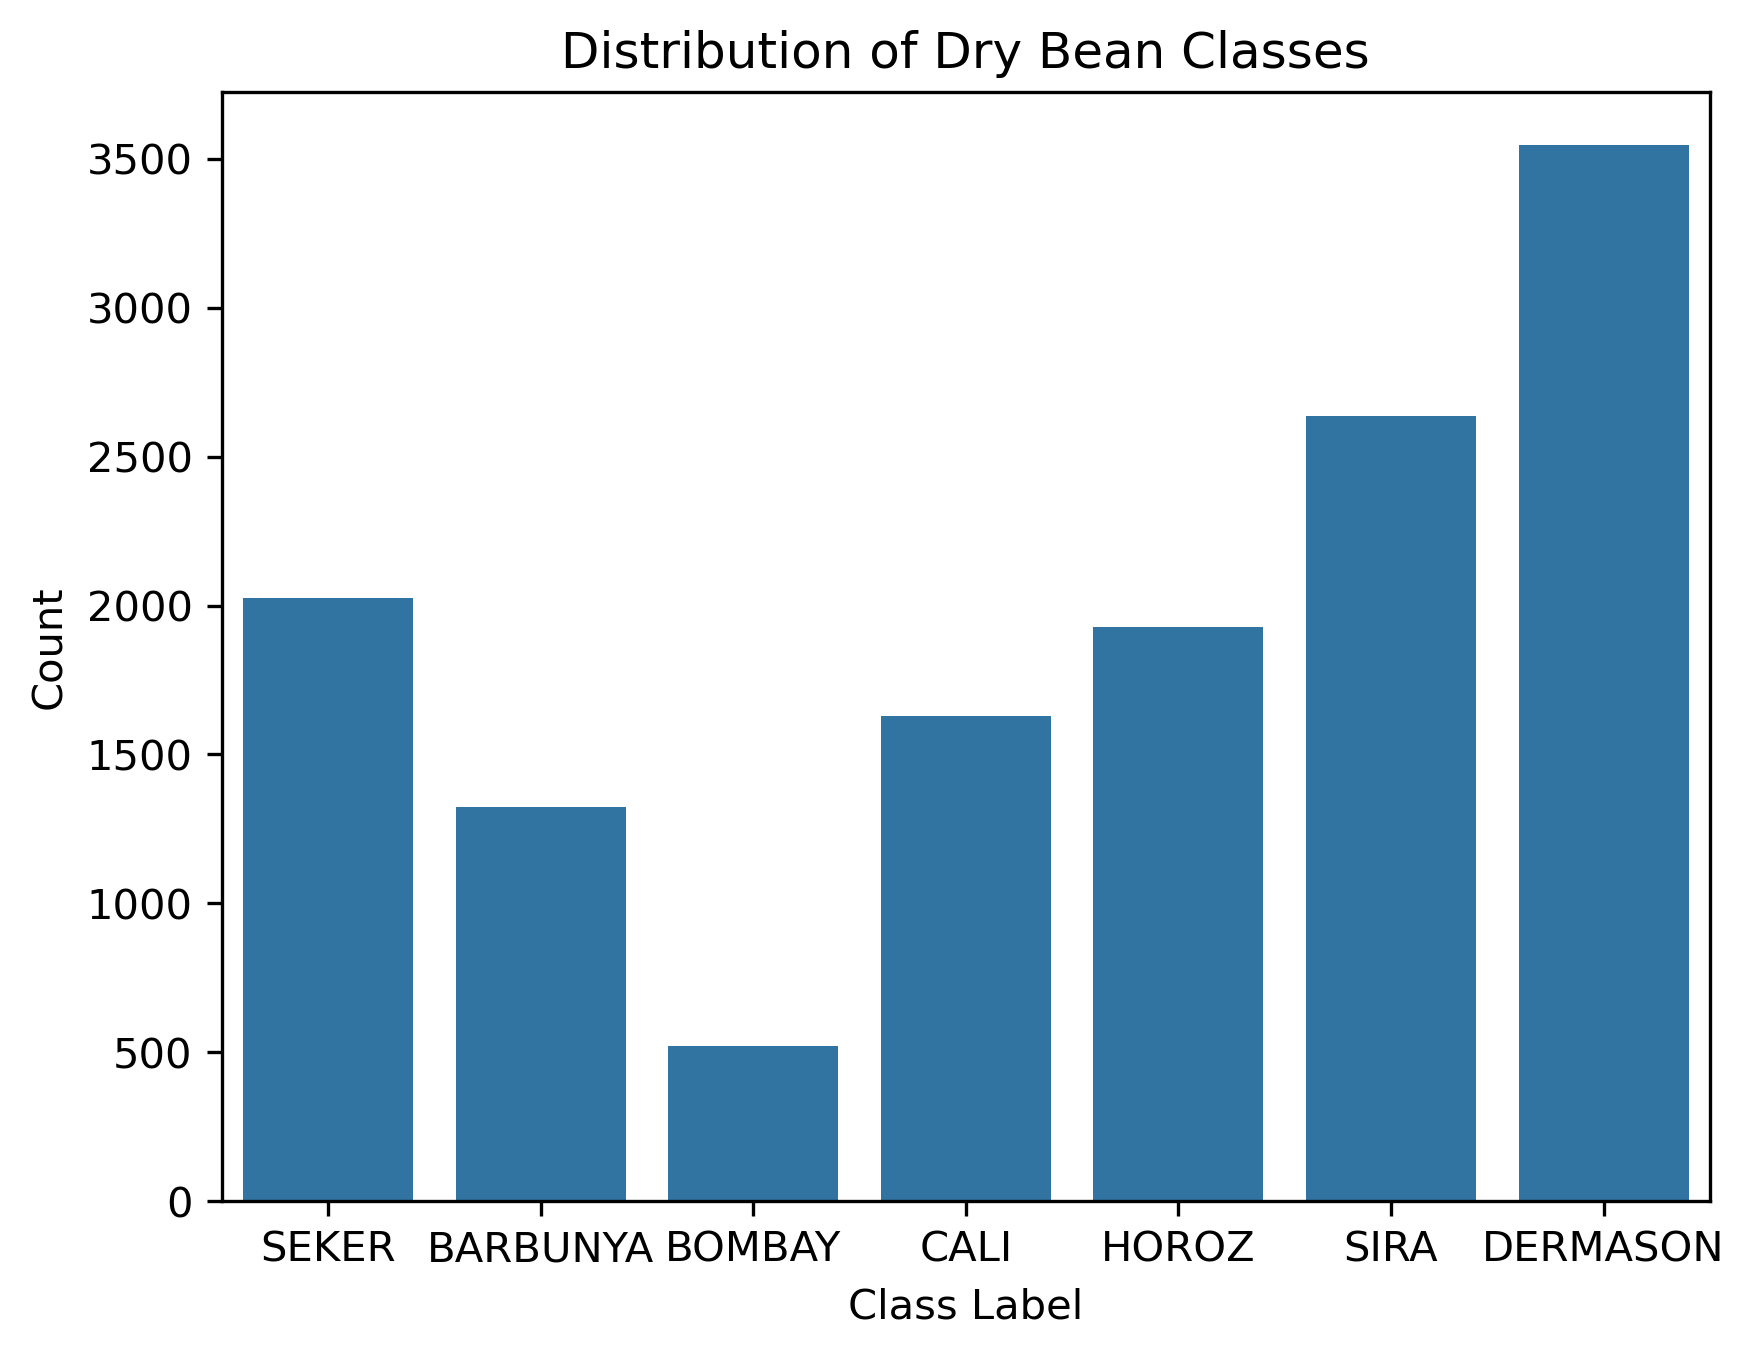
\includegraphics[width=\linewidth, height=4cm]{figures/dry_bean_class_distribution.png}
        \caption{Dry Bean label distribution}
        \label{fig:label_distribution}
    \end{subfigure}
    \hfill
    \begin{subfigure}{0.48\textwidth}
        \centering
        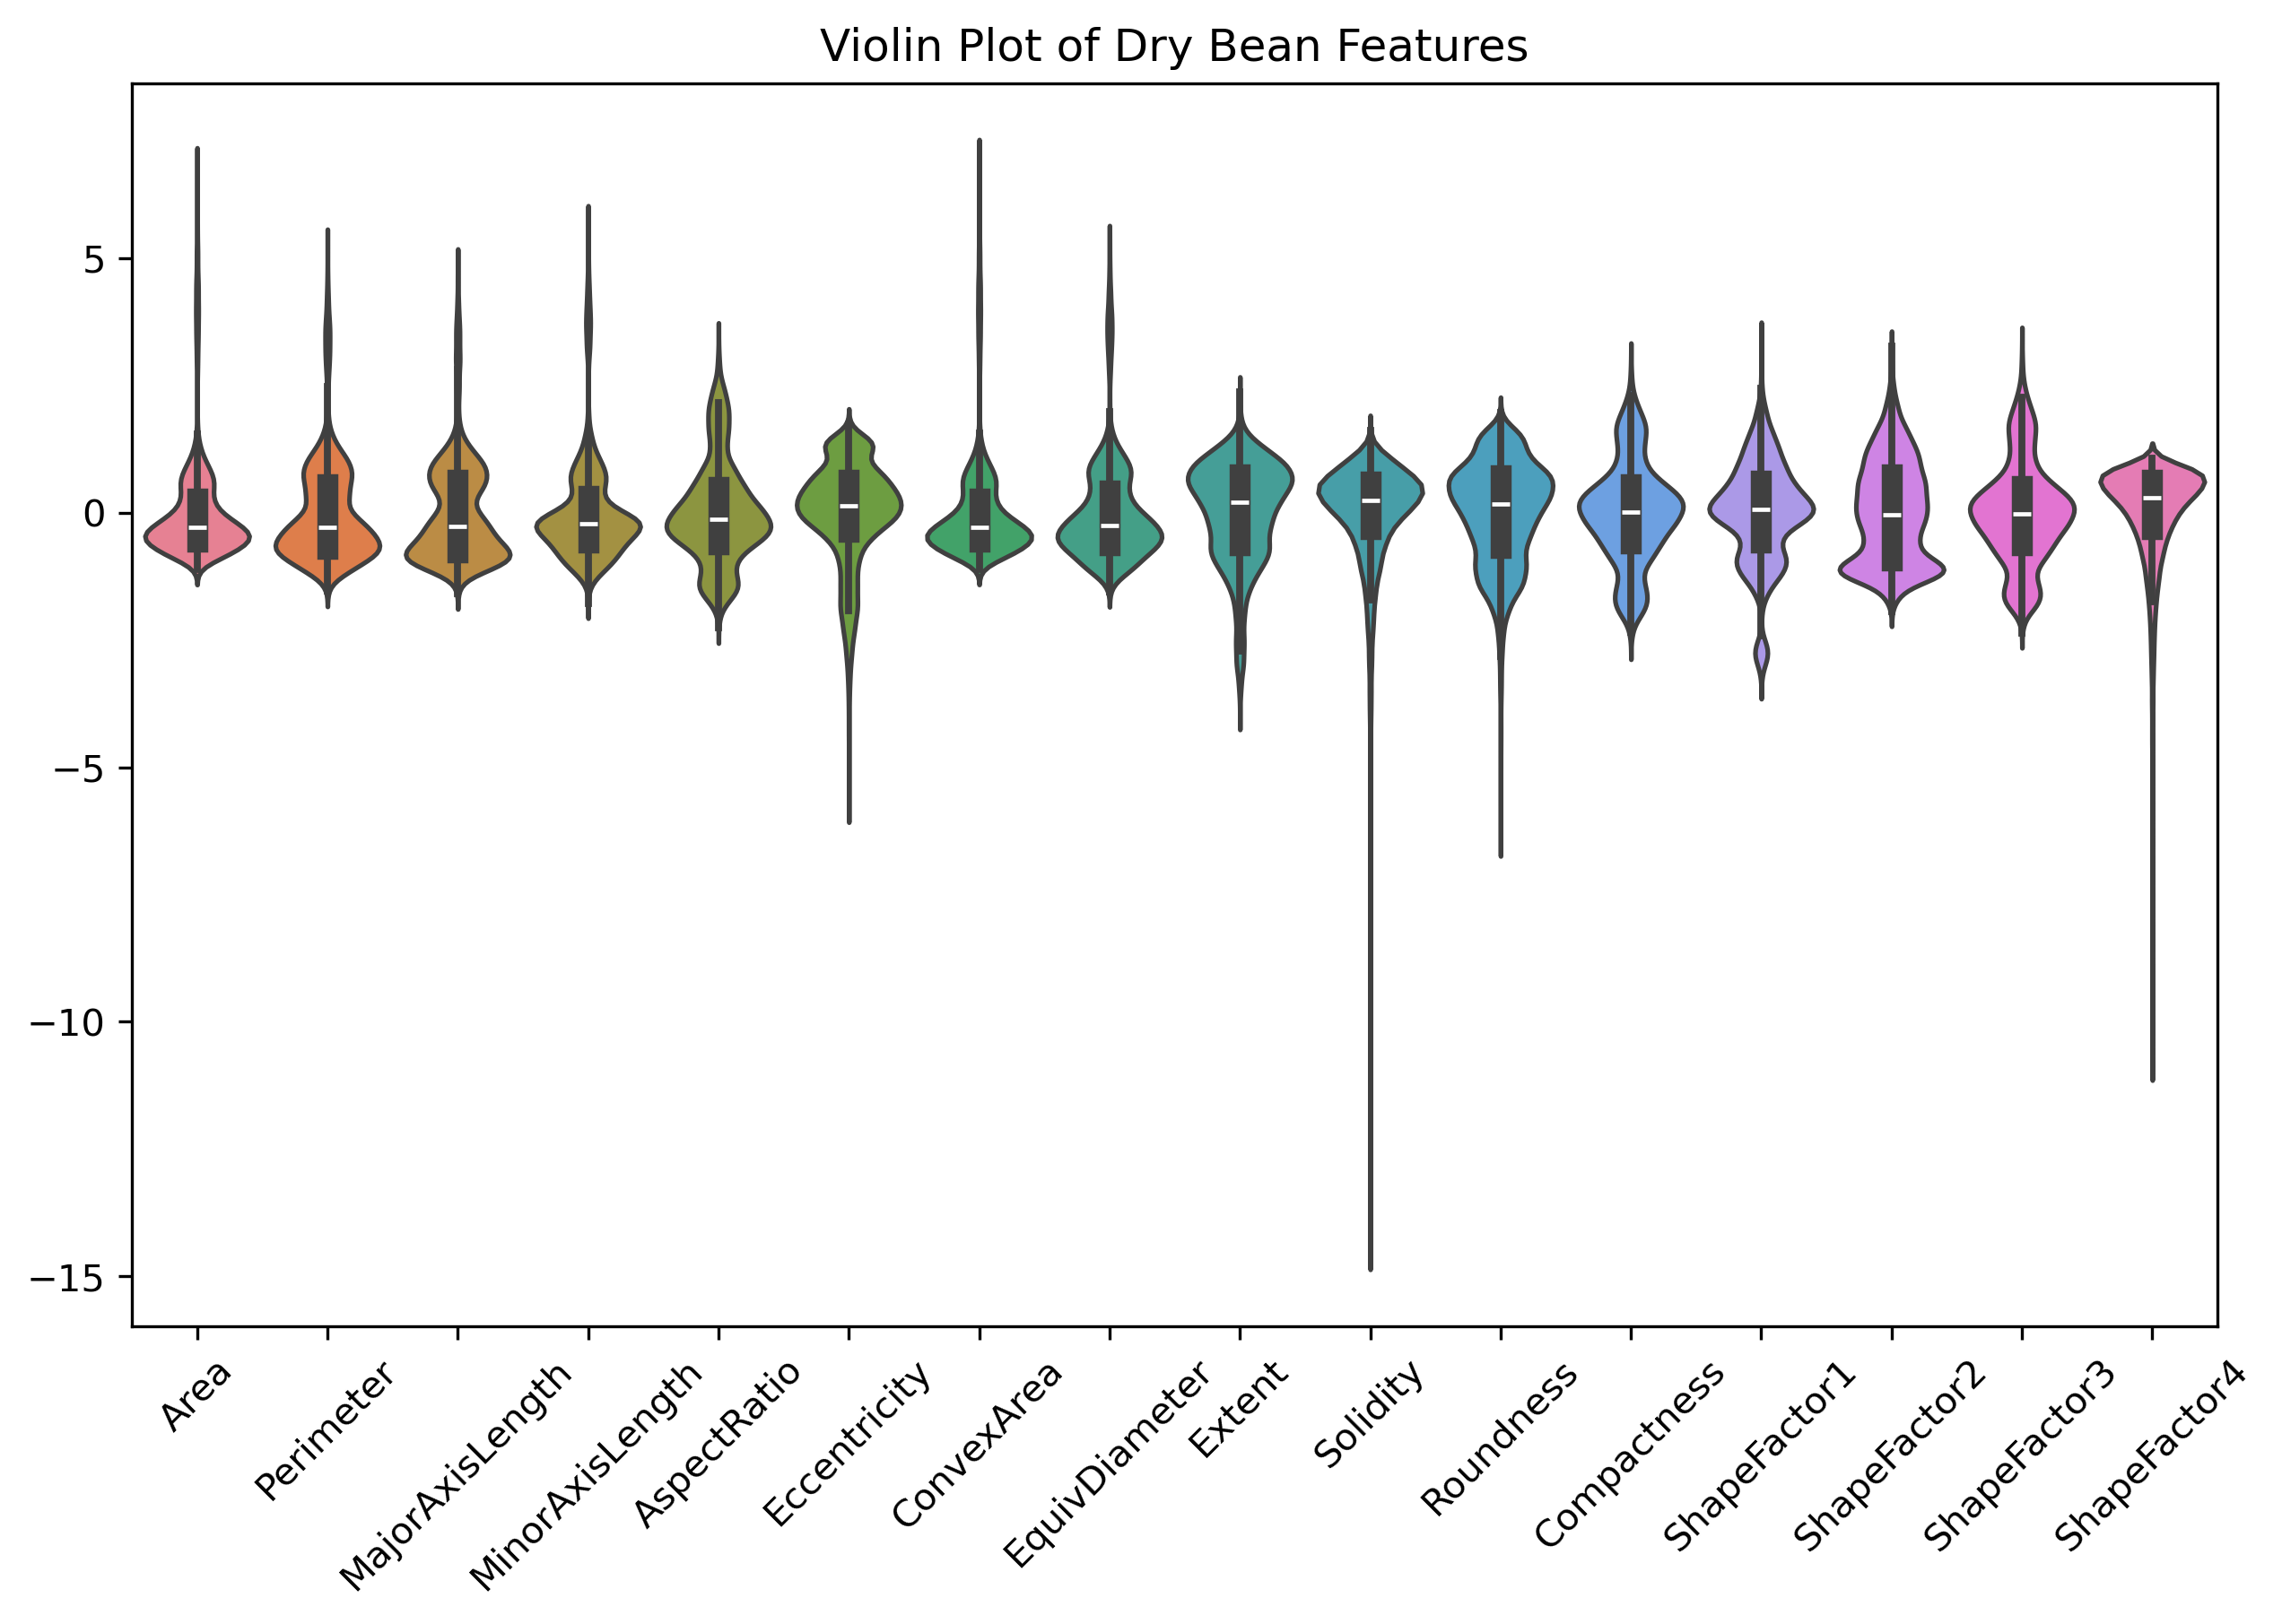
\includegraphics[width=\linewidth, height=4cm]{figures/dry_bean_violin.png}
        \caption{Violin plot of Dry Bean features}
        \label{fig:dry_bean_violin}
    \end{subfigure}
    \caption{Feature distribution of Dry Bean dataset}
    \label{fig:iris_features}
\end{figure}

\begin{figure}[h]
    \centering
    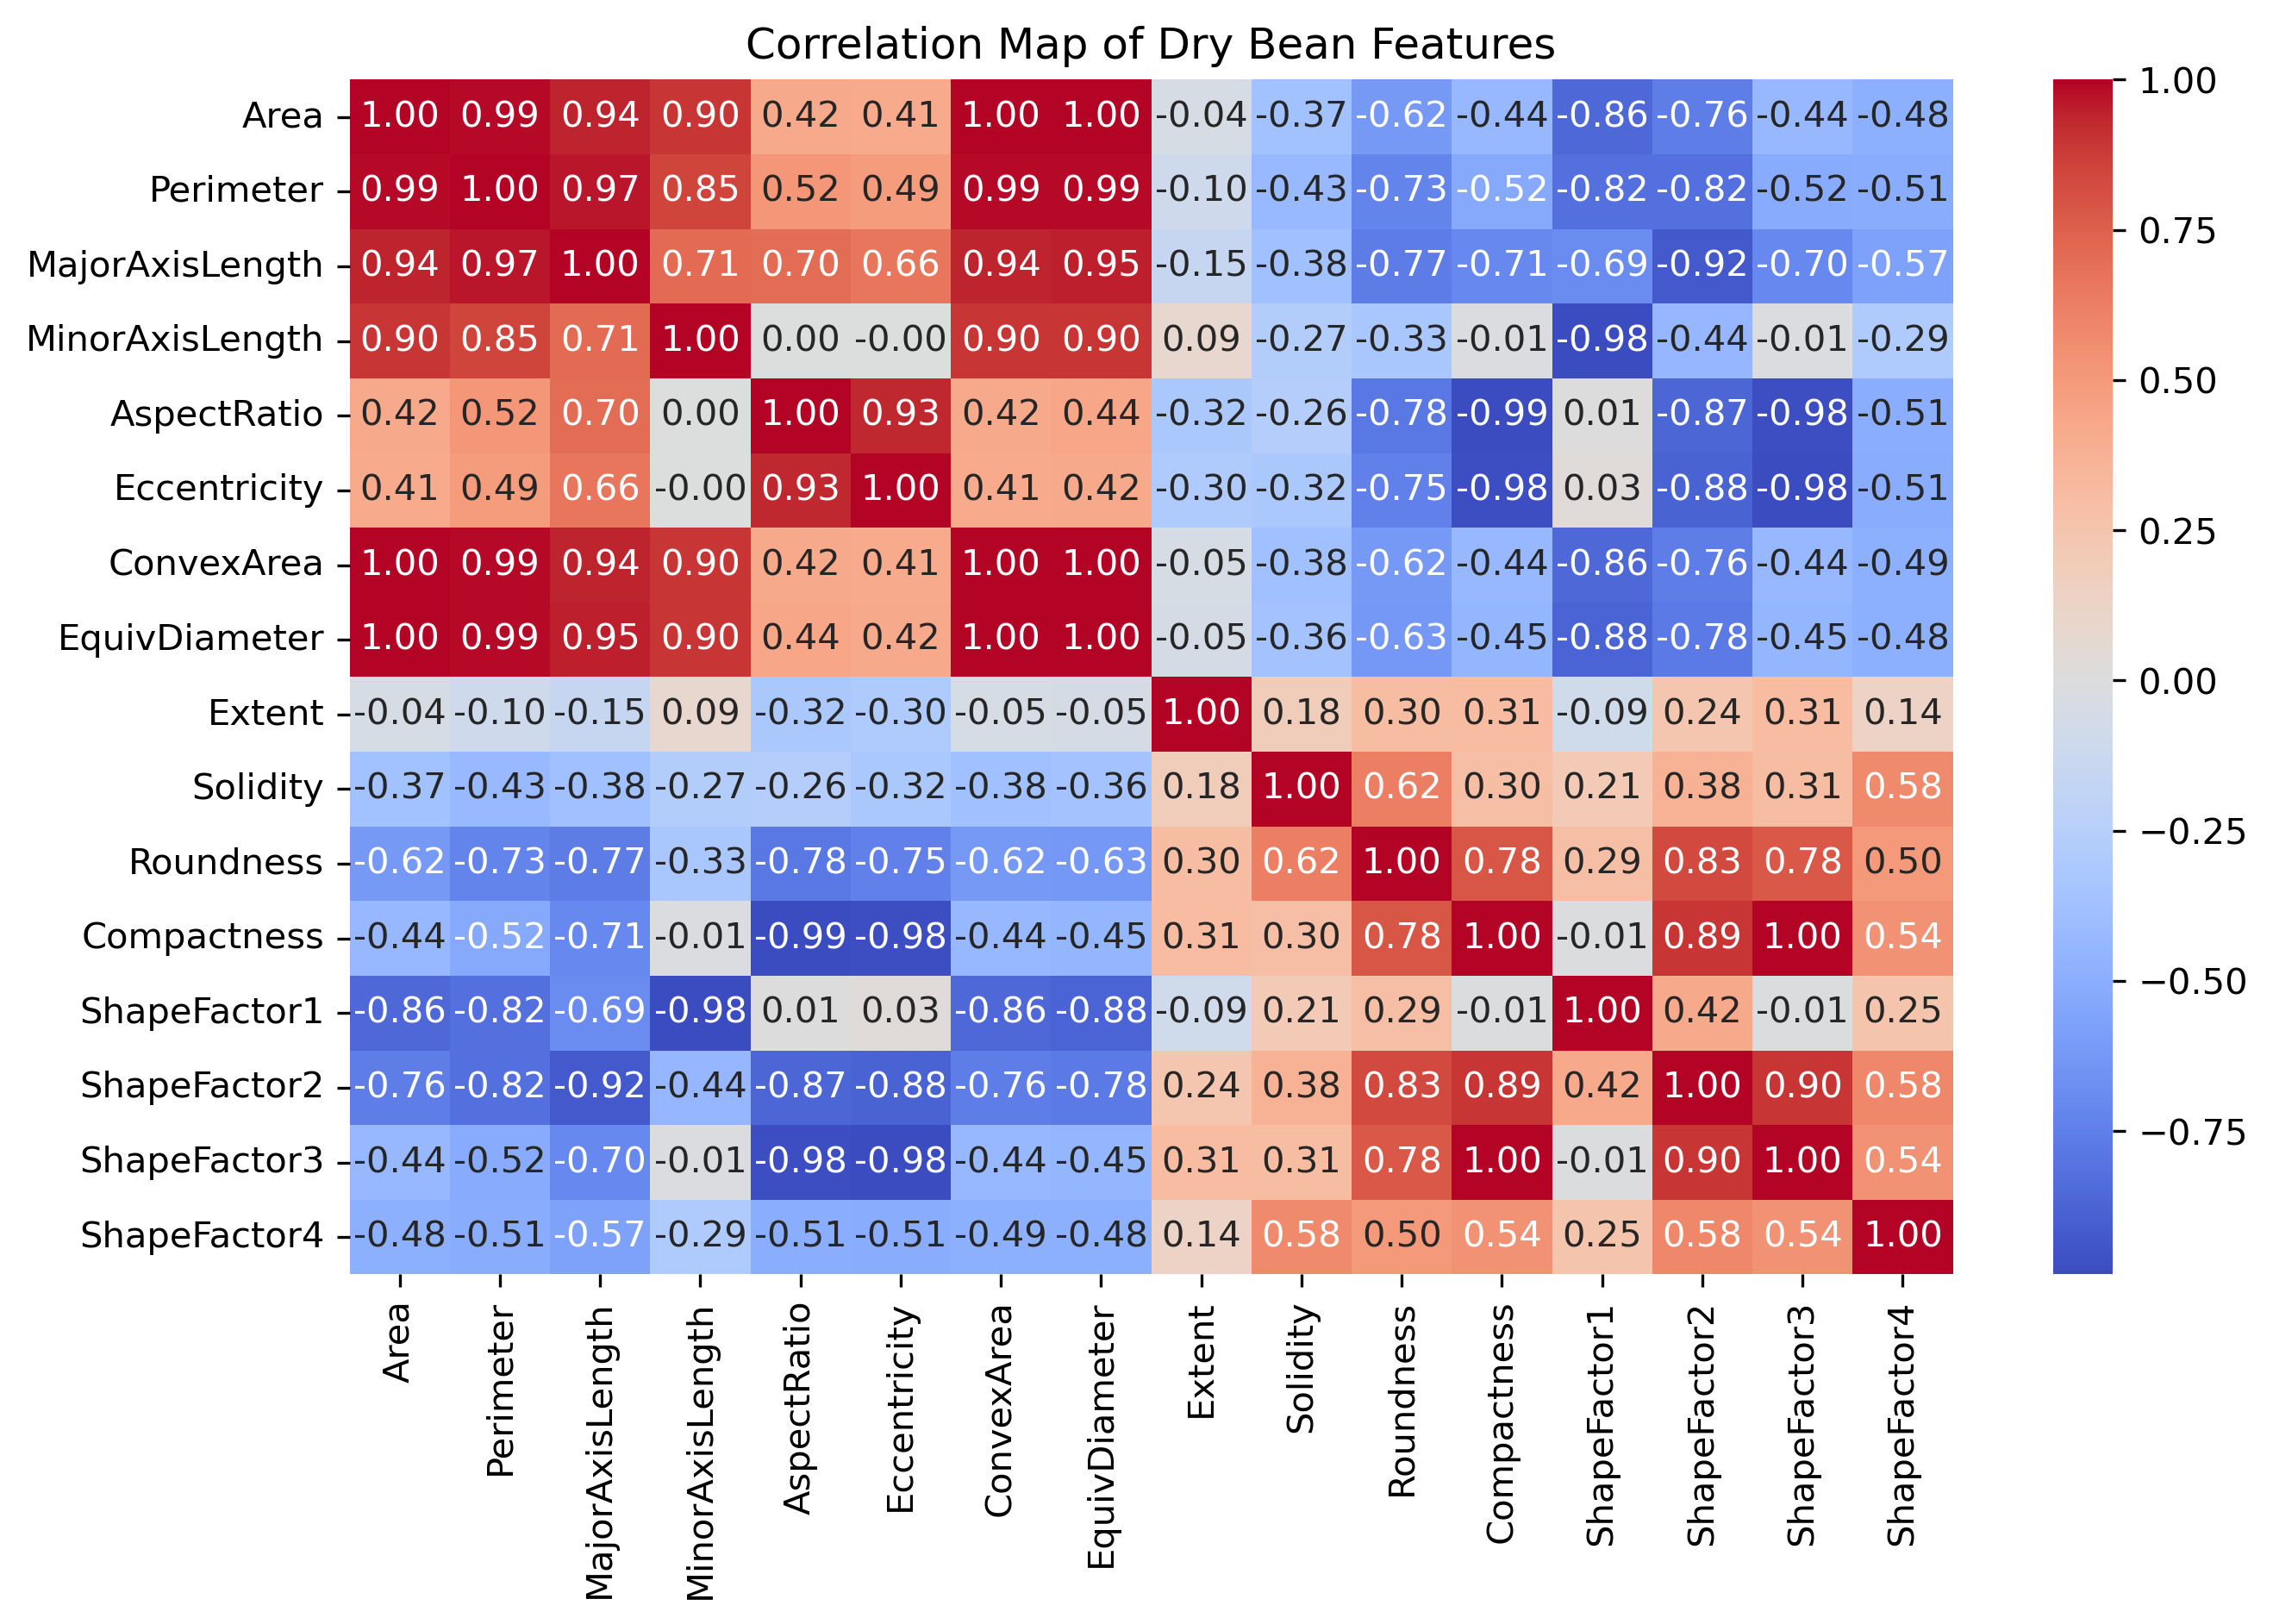
\includegraphics[width=0.8\textwidth]{figures/dry_bean_correlation.png}
    \caption{Feature correlation of Dry Bean dataset}
    \label{fig:feature_correlation}
\end{figure}

\begin{figure}[h]
    \centering
    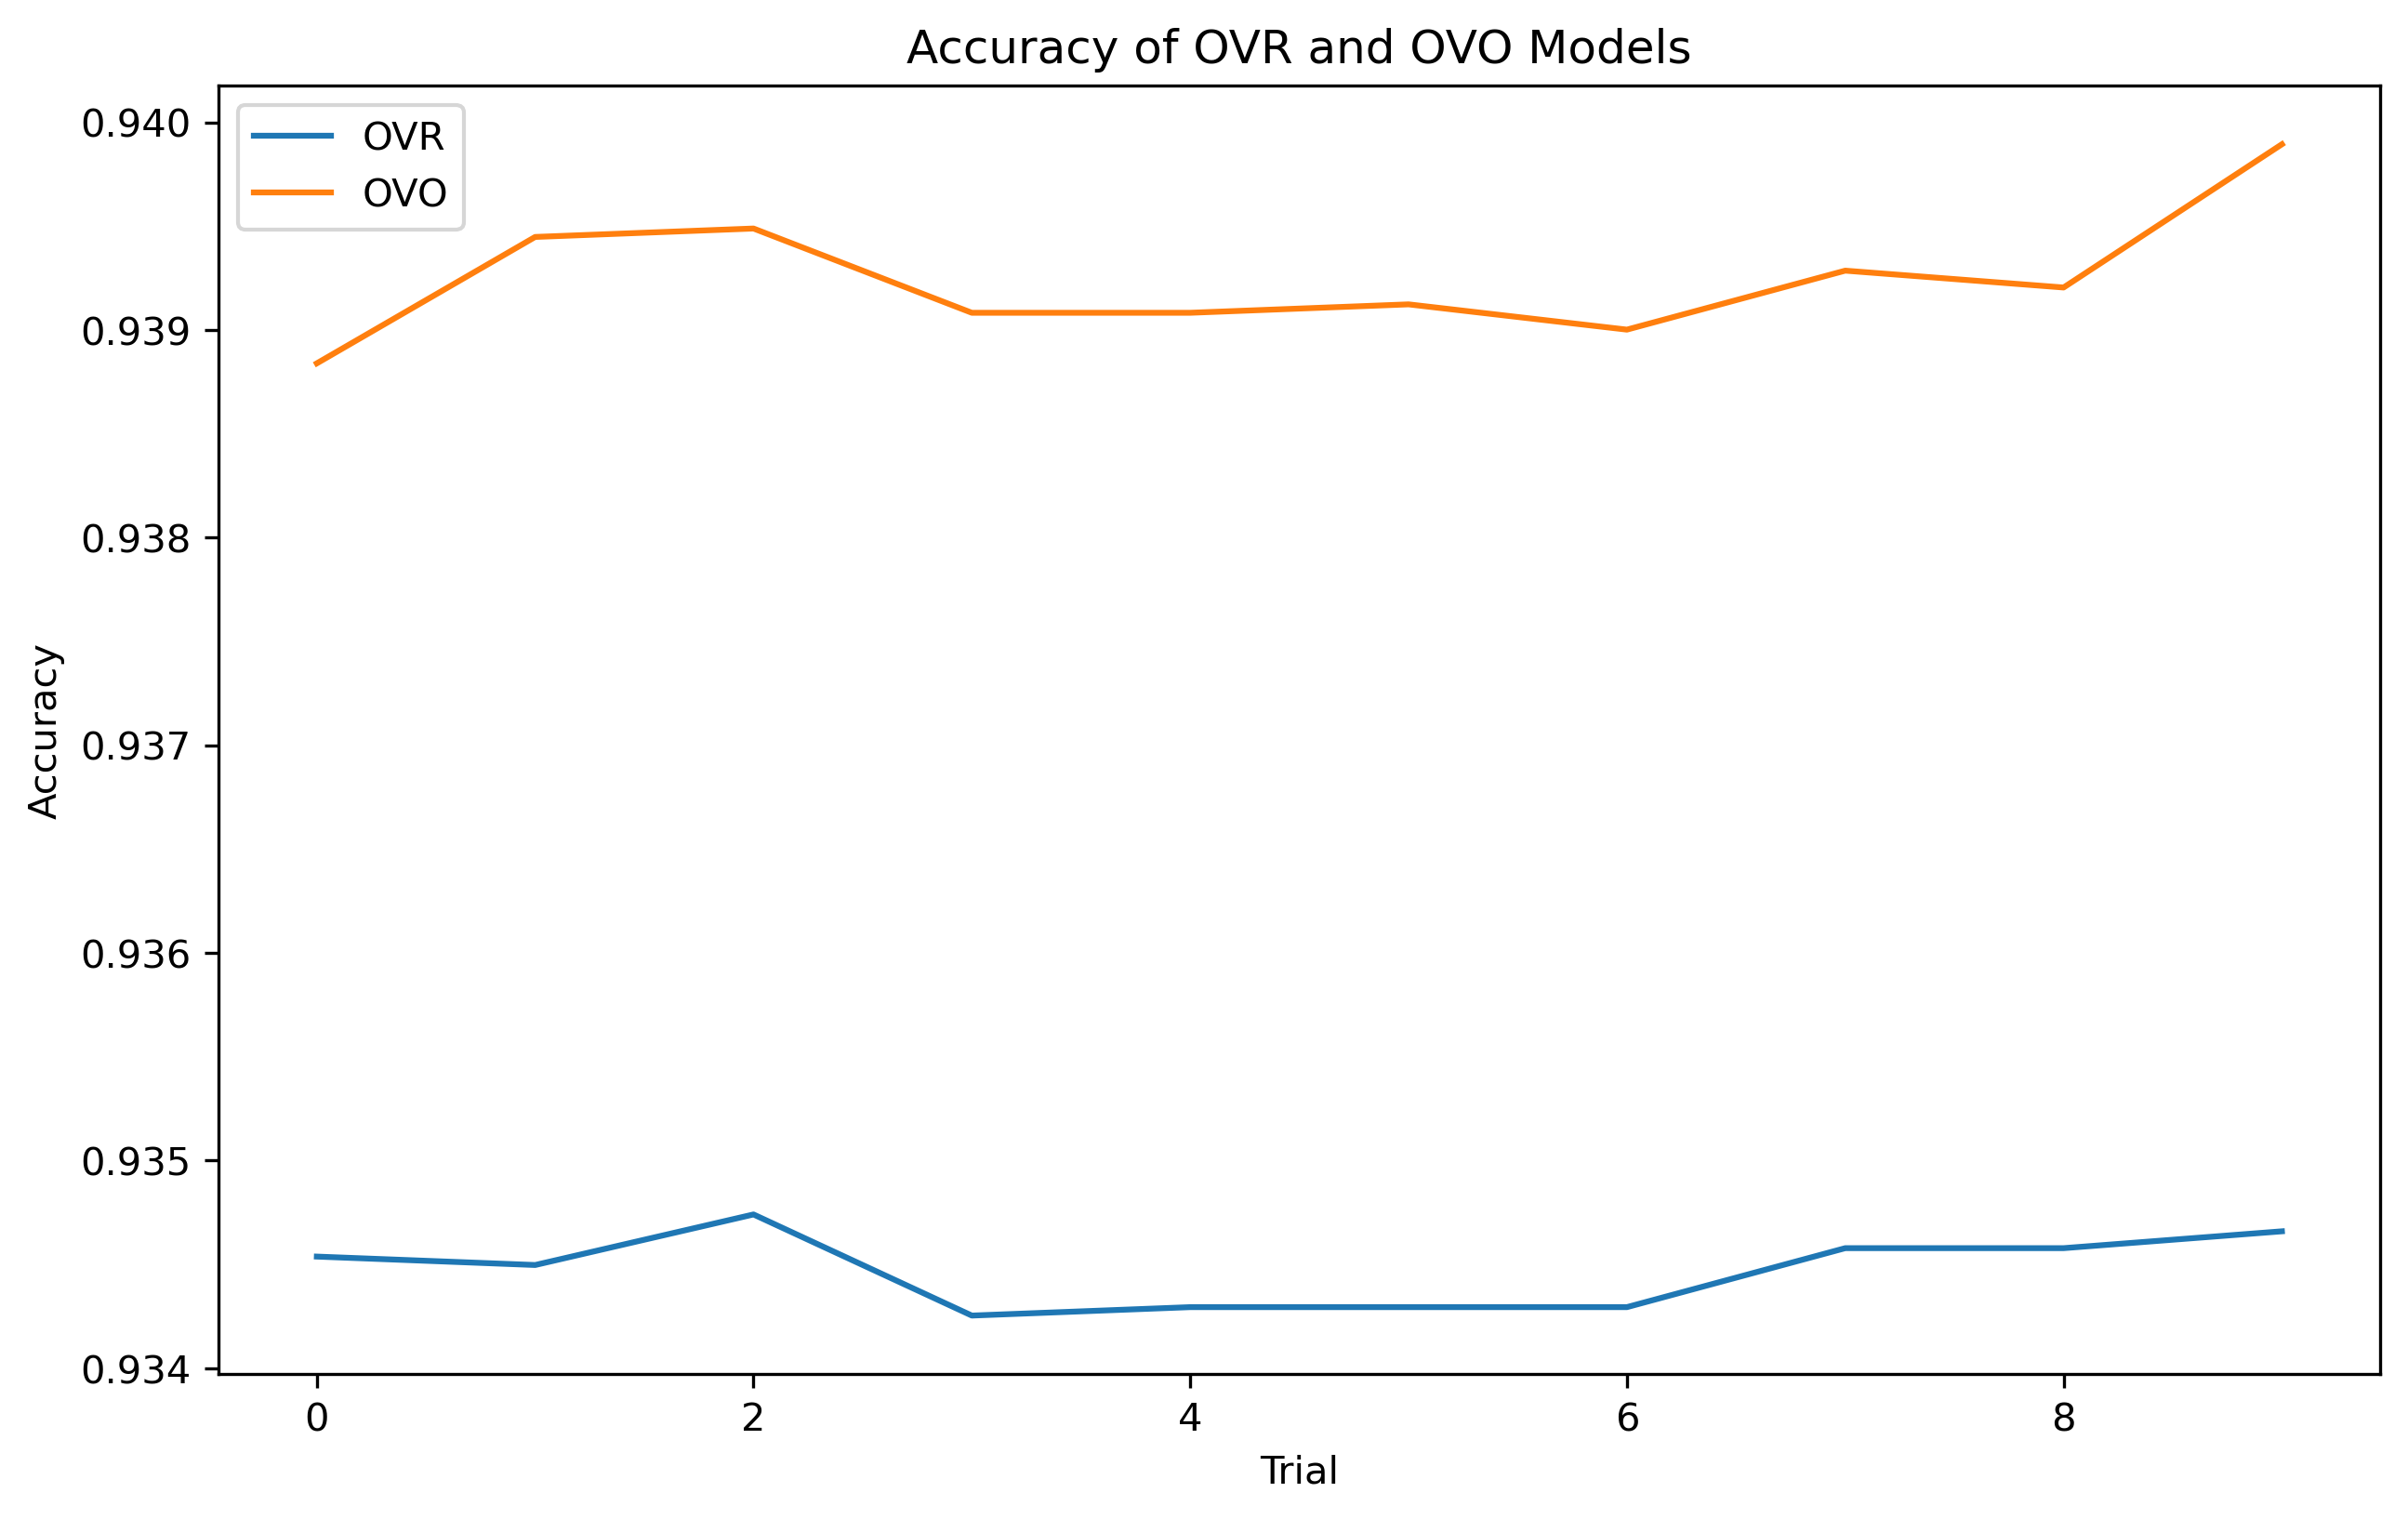
\includegraphics[width=0.8\textwidth]{figures/dry_bean_ovo_ovr_accuracy.png}
    \caption{Accuracy of Dry Bean dataset with OvO and OvR}
    \label{fig:dry_bean_accuracy}
\end{figure}

\end{document}